% =====================================================================
%  Figure captions for: honjo, a Cheminformatics DSL
%
%  Every quantity quoted below is read from
%  validation/results/exp_honjo.json.
% =====================================================================

\begin{figure*}[!htbp]
    \centering
    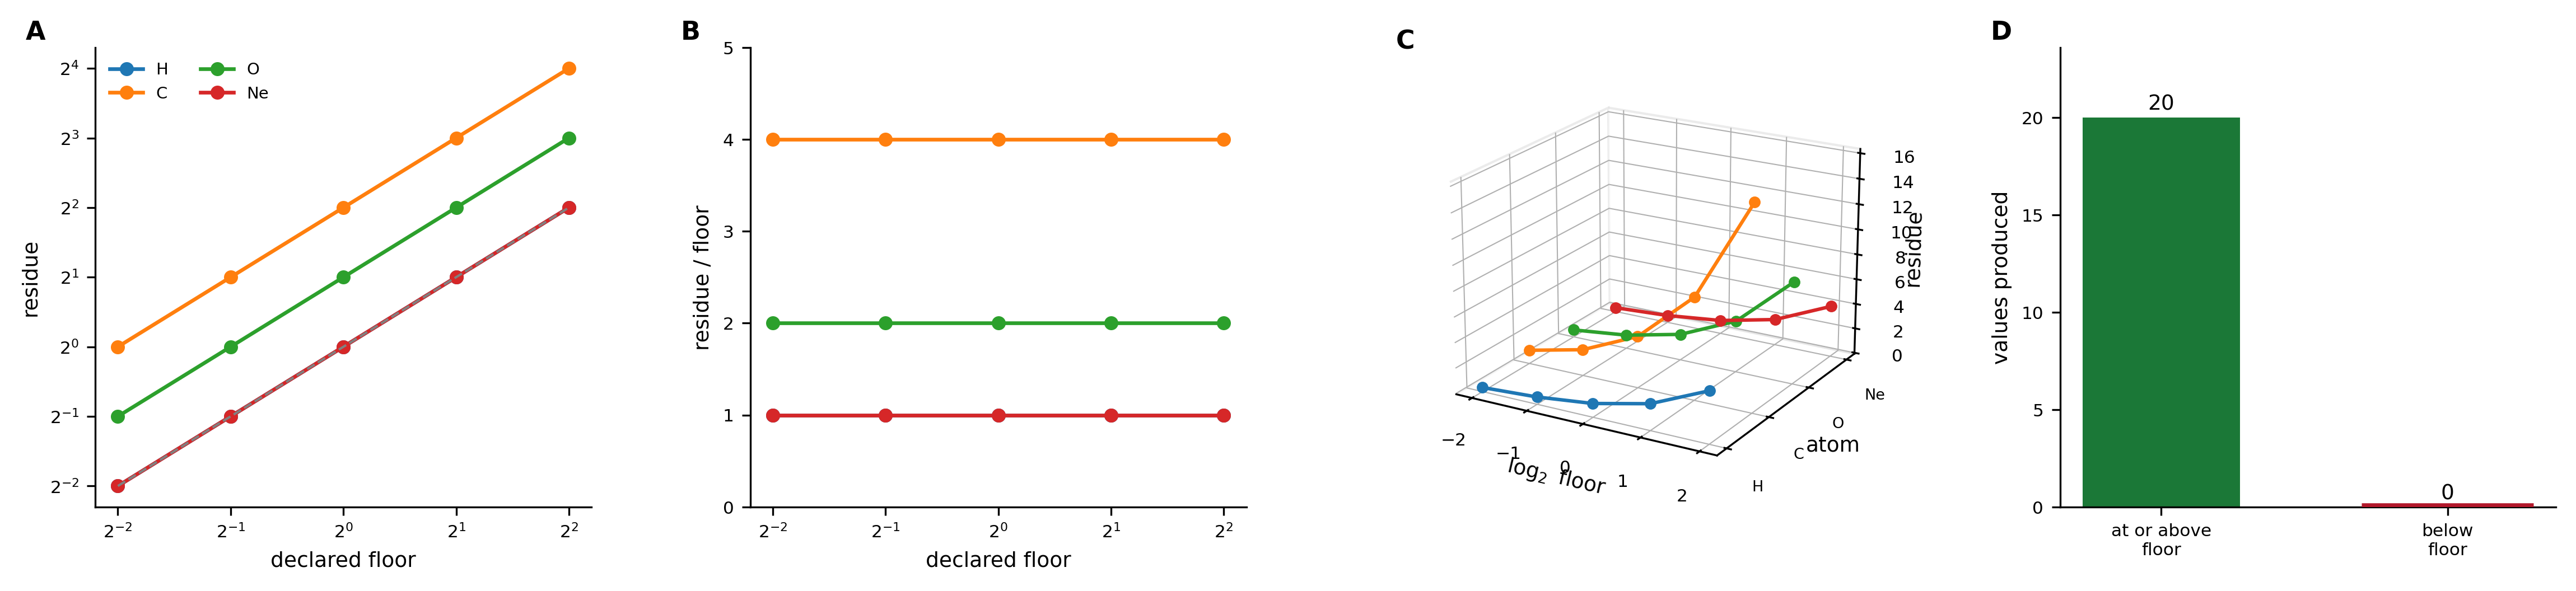
\includegraphics[width=\textwidth]{figures/panel_01_floor.png}
    \caption{\textbf{The floor is a resolution scale the value is
    expressed in, not a truncation applied to a value computed
    independently of it.}
    Conformance item (C1) asks that no program produce a value with
    $\res<\flo$. As \Cref{rem:c1-vacuous} records, that test cannot fail:
    the residue is computed as $\flo\times\nu$ under a $\max(\cdot,\flo)$
    clamp, so a sub-floor value is unconstructible. The informative
    measurement is how the residue \emph{responds} to the floor, which is
    what this panel shows.
    (\textbf{A})~Residue against declared floor on log--log axes for four
    atoms, with the identity dashed. Every trace is a straight line of
    unit slope over a sixteen-fold sweep, $\flo\in\{0.25,\dots,4\}$;
    hydrogen and neon coincide because both have unit multiplier.
    (\textbf{B})~The same data as the ratio $\res/\flo$. Each atom is flat
    across the entire sweep --- $1.0$ for hydrogen, $4.0$ for carbon,
    $2.0$ for oxygen, $1.0$ for neon. Flatness is the claim: a truncation
    applied after the fact would produce a ratio that moved with the
    floor, rising toward $1$ as the floor overtook the value.
    (\textbf{C})~The full sweep in (floor, atom, residue) space. The
    surface is ruled: for fixed atom the residue is linear in the floor,
    and for fixed floor it is a per-atom multiple. Those two facts
    together are what ``the floor is a resolution'' means operationally.
    (\textbf{D})~Values at or above the floor against values below it,
    over all $20$ runs of the sweep. The below-floor count is zero, drawn
    as an explicit floor tick. We report it alongside
    panel~(\textbf{B}) rather than alone, because on its own it is a
    restatement of the clamp rather than evidence about the language.}
    \label{fig:floor}
\end{figure*}

\begin{figure*}[!htbp]
    \centering
    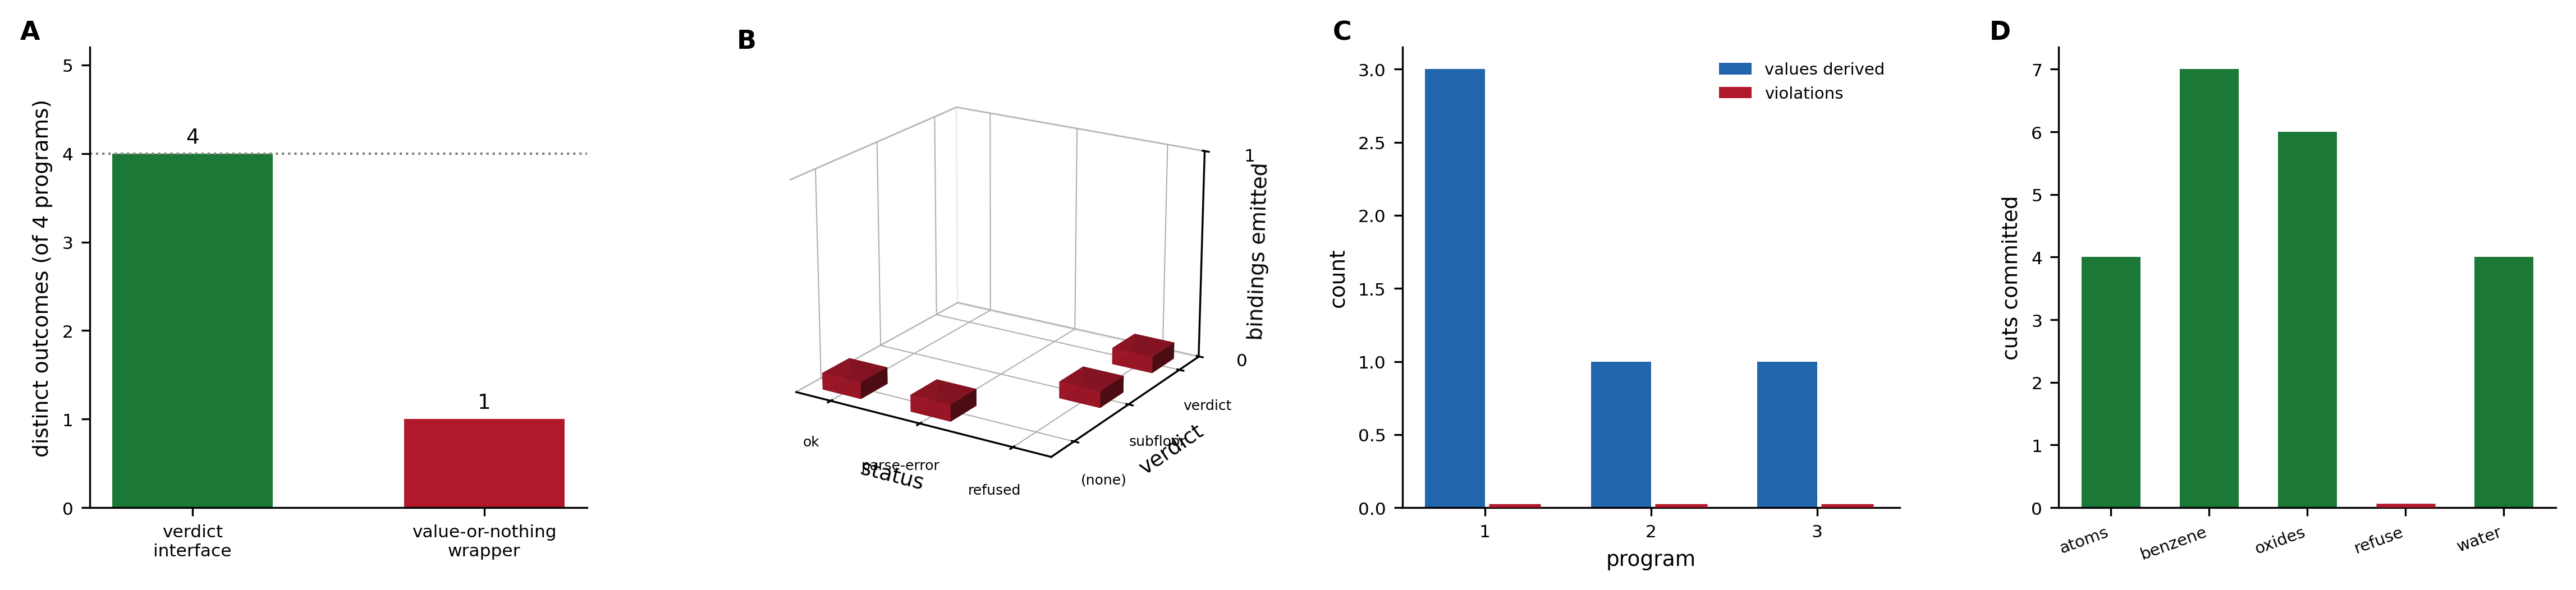
\includegraphics[width=\textwidth]{figures/panel_02_conflation.png}
    \caption{\textbf{Four programs failing for four different reasons are
    four outcomes under the verdict interface and exactly one under a
    value-or-nothing wrapper.}
    The four are a sub-resolution floor, a parse error, an unbound
    reference, and an import refused on provenance.
    \Cref{rem:c4-programs} records why \hj{unclosed} and \hj{inert} are
    not among them: both bind values, so both report \emph{value} under
    the wrapper and would make the control fail for the wrong reason.
    (\textbf{A})~Distinct outcomes under each interface. The verdict
    interface distinguishes all four; the wrapper returns one. That
    collapse is what makes \Cref{thm:conflation} non-vacuous on this
    implementation --- exhibited rather than assumed.
    (\textbf{B})~Each program placed by status and verdict kind, with
    height the number of bindings emitted. All four sit at zero height:
    they occupy four distinct positions in the (status, verdict) plane and
    the same position on the value axis, which is precisely the geometry
    the theorem describes.
    (\textbf{C})~Provenance monotonicity (C2), a separate measured item.
    Values derived per program against violations found. The violation
    count is zero in every program, drawn as explicit floor ticks.
    Composition is maximum, so a $\supplied$ input can never yield a
    $\stated$ output; a violation would be convention laundered into
    record.
    (\textbf{D})~Cuts committed by each example program, coloured by
    whether the program completed. \hj{refuse.hj} commits none, because it
    declines before measuring anything: a refusal costs no cuts, which is
    the operational content of refusing rather than computing and
    discarding.}
    \label{fig:conflation}
\end{figure*}

\begin{figure*}[!htbp]
    \centering
    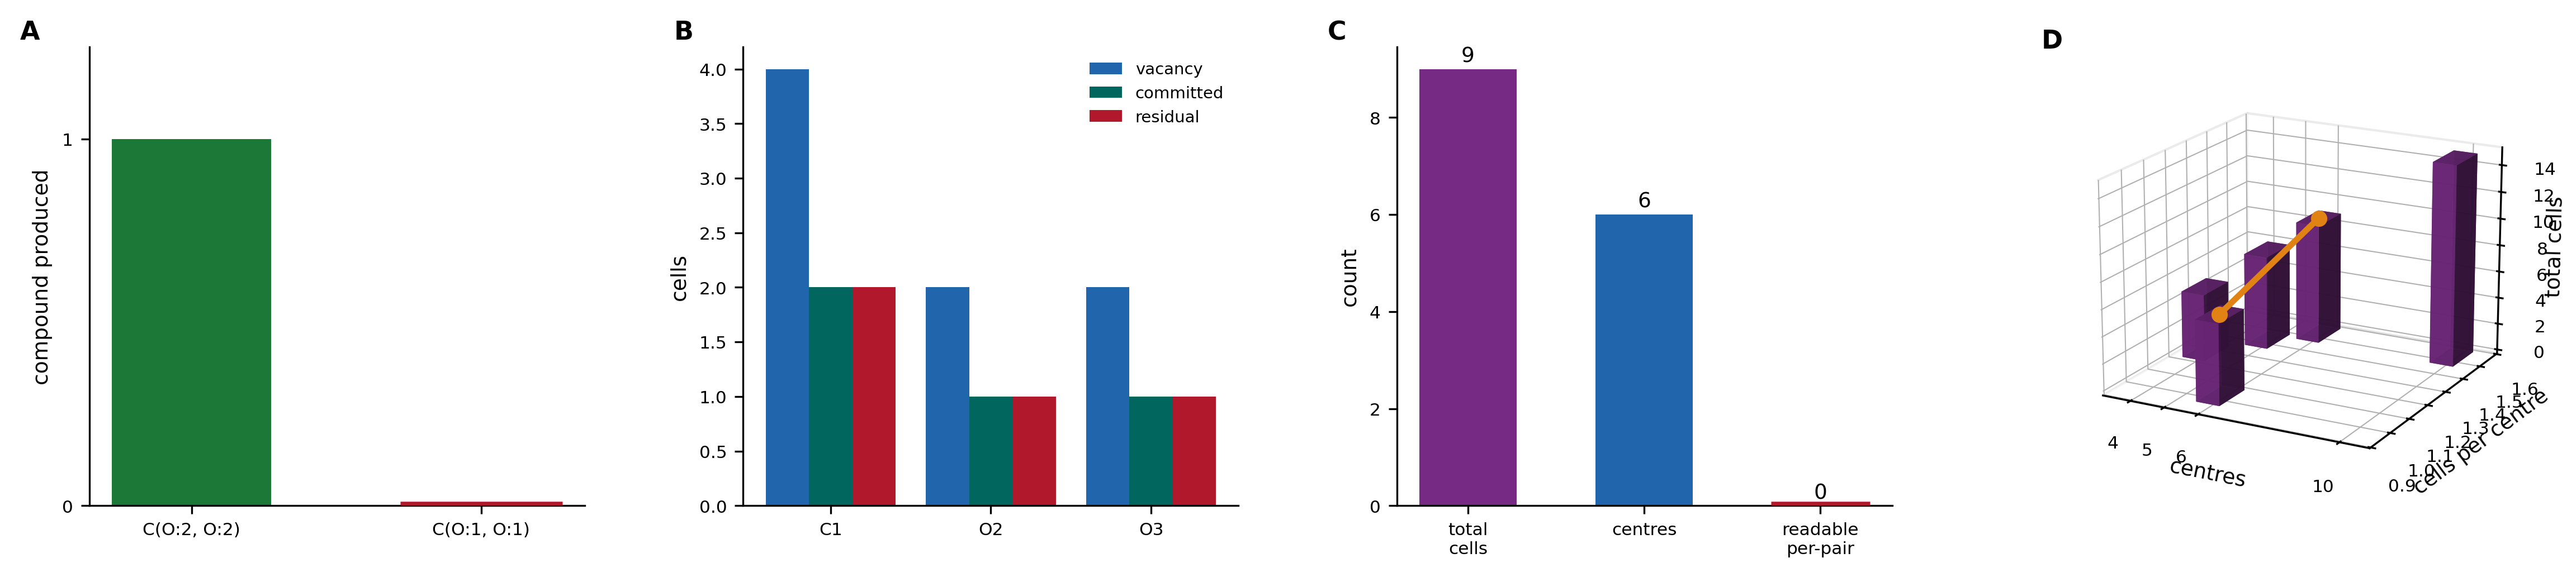
\includegraphics[width=\textwidth]{figures/panel_03_cells.png}
    \caption{\textbf{Committed cell counts change what is built, and a
    delocalised system carries a total that no per-pair count can be
    recovered from.}
    (\textbf{A})~The same atoms at the same stoichiometry under two cell
    commitments. \hj{close C(O : 2, O : 2)} produces a compound;
    \hj{close C(O : 1, O : 1)} produces none, drawn as an explicit zero.
    The difference is stronger than a differing field: one program yields
    a value and the other yields a verdict.
    (\textbf{B})~Why the one-cell reading yields nothing: vacancy,
    committed cells and residual per atom in the \textsf{unclosed}
    verdict. Carbon has vacancy $4$ with $2$ committed, leaving residual
    $2$; each oxygen leaves $1$. A connectivity-only model writes both
    programs as ``carbon bonded to two oxygens'' and cannot express the
    difference, which is conformance item (C5).
    (\textbf{C})~The benzene delocalised system: total cells $9$ over $6$
    centres, and zero readable per-pair values. The implementation names
    a \textsf{per\_pair\_cells} field and holds it null, which we take to
    be the stronger choice --- the absence is declared rather than left
    to be inferred from a missing key. What (C6) forbids is a readable
    count, and none is readable.
    (\textbf{D})~Five delocalised systems the interpreter actually built,
    positioned by centre count and cells per centre, with height the
    total. The orange spine joins the two systems that share a centre
    count of $6$ and carry different totals, $6$ and $9$. Because the
    total is not a function of the centres, it cannot be unpacked into a
    per-pair count by dividing --- which is why (C6) is a claim about the
    value rather than a convention about its presentation.}
    \label{fig:cells}
\end{figure*}

\begin{figure*}[!htbp]
    \centering
    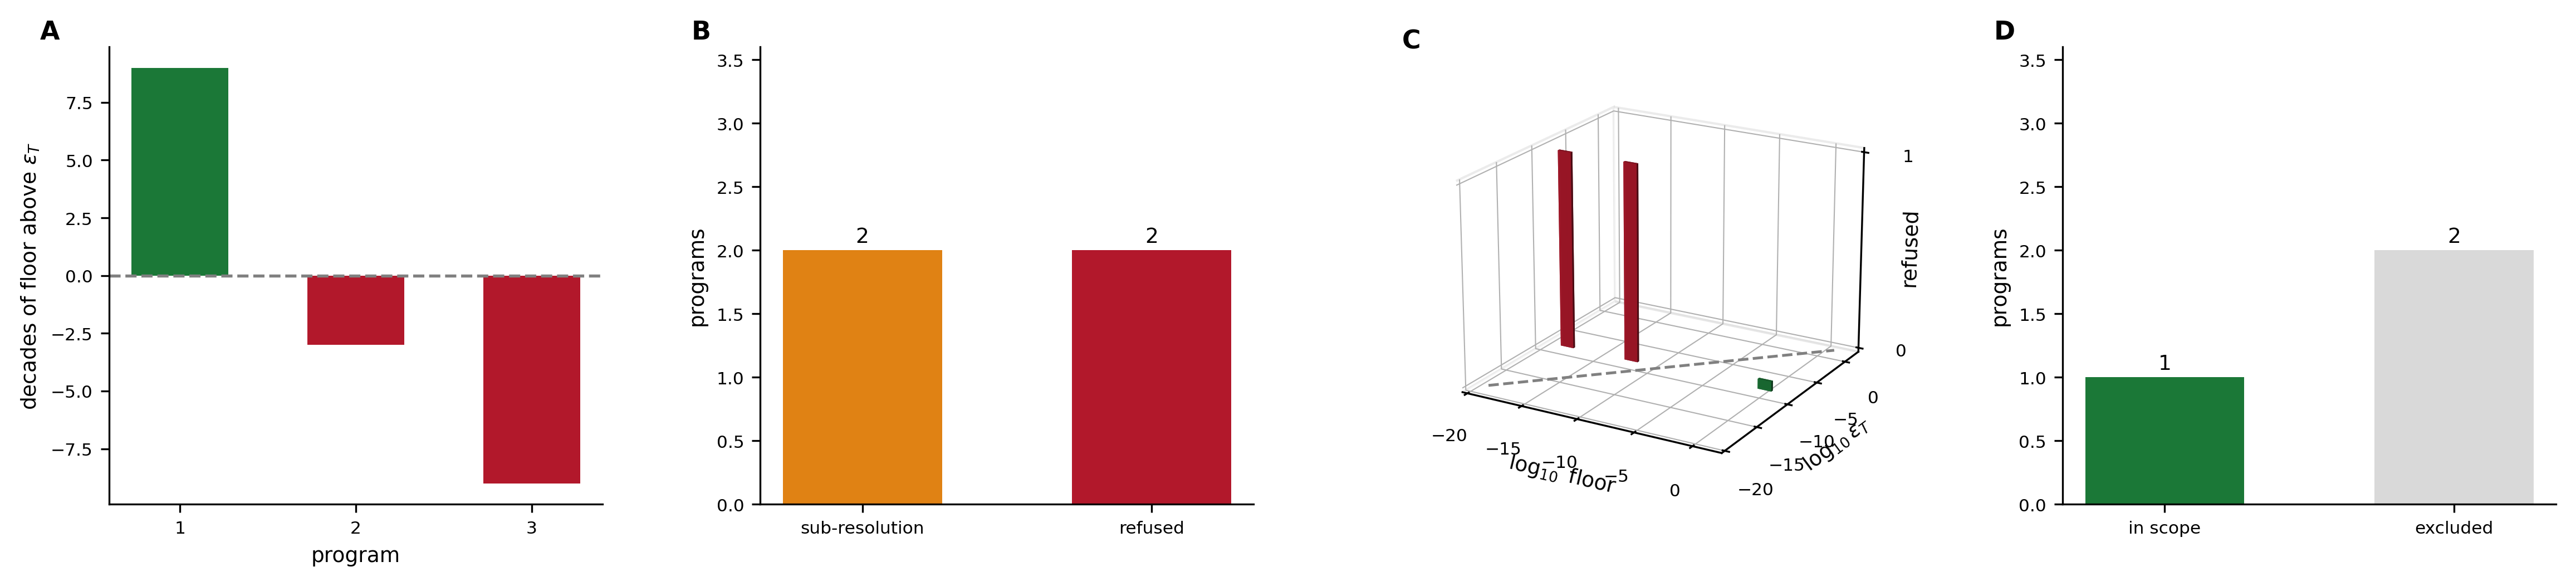
\includegraphics[width=\textwidth]{figures/panel_04_resolution.png}
    \caption{\textbf{A floor finer than the target's resolution is
    refused with both numbers named, and the refused programs are
    excluded from the equivalence claim rather than run and tolerated.}
    (\textbf{A})~Each program's declared floor as decades above the
    target resolution $\eps_T=10^{-9}$, with the gate at zero. One
    program clears it; two fall $3$ and $9$ decades below. The axis is a
    margin rather than a raw $\log_{10}$ floor because the raw quantity
    renders the single admitted program (floor $1.0$, $\log_{10}=0$) as an
    invisible bar while the refused ones become large spikes, which reads
    backwards.
    (\textbf{B})~Programs below the resolution against programs refused.
    The two counts are equal at $2$: the gate fires on exactly the
    programs that trip it, neither over- nor under-refusing.
    (\textbf{C})~The gate in (floor, target resolution, refused) space
    with the line $\flo=\eps_T$ drawn. Bars stand at height $1$ on the
    sub-resolution side and lie flat on the other. The refusal verdict
    carries both numbers, the declared $10^{-12}$ and the target
    $10^{-9}$; \Cref{rem:ambient} notes that the declared value lives in
    the verdict rather than in the interpreter's ambient state, since a
    refused declaration by definition did not take effect.
    (\textbf{D})~Scope of \Cref{thm:target-equiv}: one program in scope,
    two excluded. The in-scope set is a strict subset, which is the
    discipline \Cref{rem:c8} asks for --- a suite that ran the excluded
    programs on both back ends and reported their disagreement as
    tolerable would be asserting the unconditional theorem that
    \Cref{rem:equiv-honest} retracts.}
    \label{fig:resolution}
\end{figure*}
